\documentclass[../main.tex]{subfiles}
\graphicspath{{\subfix{../images/}}}
\begin{document}


\section{Neúplné LU rozklady (ILU - incomplete LU decomposition)}

Při LU rozkladu vzniká zaplnění, LU rozklad se počítá "přibližně" a ignorují se některá (nebo všechna)
zaplnění. Takováto aproximace $\tilde{\mathbb{L}}\tilde{\mathbb{U}}\approx \mathbb{A}$ může sloužit jako účinné předpodmínění.

\subsection{ILU(k)}

Pro SPD matice můžeme použít neúplný Choleského rozklad (IC - Incomplete Cholesky). Základní varianta ILU(0), resp. IC(0).\\
LU rozklad po řádkách:

\begin{minipage}{0.95\linewidth}
    \begin{verbatim}
    for i = 2 ... n 
        for k = 1 ... i-1
            a_{ik} = a_{ik}/a_{kk}
            for j = k+1 ... n
                a_{ij} = a_{ij} - a_{ik}a_{kj}
            end j 
        end k 
    end i
    \end{verbatim}    
\end{minipage}


Z toho dostáváme ILU(0):

\begin{minipage}{0.95\linewidth}
    \begin{verbatim}
    for i = 2 ... n 
        for k = 1 ... i-1
            if a_{ik} != 0
                a_{ik} = a_{ik}/a_{kk}
                for j = k+1 ... n
                    if a_{ij} != 0
                        a_{ij} = a_{ij} - a_{ik}a_{kj}
                    end if
                end j
            en dif  
        end k 
    end i
    \end{verbatim}    
\end{minipage}

Výsledkem je matice  se stejnou strukturou jako původní matice, vzniká nulové zaplnění.


Obecněji lze předepsat $P \subset \hat{n} \times \hat{n}$ ve kterých zanedbáváme zaplnění
\begin{equation*}
    P = \left\{ (i,j) \in \hat{n} \times \hat{n} | l_{ij} = 0\text{ pro i>j, respektive }u_{ij} = 0 \text{ pro } i>j  \right\}
\end{equation*}

Nesmí se zanedbávat diagonální prvky $\implies P \subset \{(i,j)\in \hat{n} \times \hat{n}, i\neq j \}$

Podmínky if v algoritmu se pak nahradí na $if(i,k)\notin P$ a $if(i,j)\notin P$, jde o neúplnost podle masky.

Platí věta:
\begin{theorem}
    Pokud \matA je M-matice a $P\subset\{(i,j)\in \hat{n} \times \hat{n}| i\neq j\}$, pak algoritmus ILU s maskou P neselže
    a sestrojí neúplný LU rozklad matice \matA tvaru $\mathbb{A} = \mathbb{L} \mathbb{U} - \mathbb{R}$, který je regulární.
    
    Metoda prosté iterace s tímto předpodmíněním bude konvergovat.
\end{theorem}

Matice $\mathbb{R}$ odpovídá zanedbaným prvkům, platí že pro $(i,j)\notin P, R_{ij} = 0$.

ILU(0) odpovídá volbě $  P = \left\{ (i,j) \in \hat{n} \times \hat{n} | a_{ij} = 0 \right\}$.

Pokud chceme přesnější LU rozklad, lze připustit i některé zaplnění, například takto:

Definujeme pro každé $(i,j)\in \hat{n} \times \hat{n} $ takzvaný $level_{ij}, level_{ij}=0$ pokud $a_{ij} \neq 0$.
Pokud při konstrukci LU rozkladu vzniká na pozici $(i,j)$ zaplnění a vzniká součinem $a_{ik} a_{kj} \neq 0$, pak definujeme
$level_{ij} = level_{ik} + level_{kj} + 1$. 

Definujeme $  P_k = \left\{ (i,j) \in \hat{n} \times \hat{n} | i\neq j \wedge level_{ij} > k \right\}$.

ILU(k) pak označuje neúplnost podle úrovně zaplnění. 


\subsubsection{Grafová interpretace ILU(k)}

Zaplnění na pozici $(i,j)$ má $level_{ij} = k \Leftrightarrow$ v $G(\mathbb{A}) \exists$ cesta z i do j vedoucí přes vrcholy s indexy $< \min\{i,j\}$ délky $k+1$.

Z toho jde předpovědět pozice zaplnění v ILU(k) (symbolická faktorizace).

\begin{remark}
    I pro ILU(1) může vznikat problém s množstvím zaplnění například


    \begin{figure}[H]
        \centering
        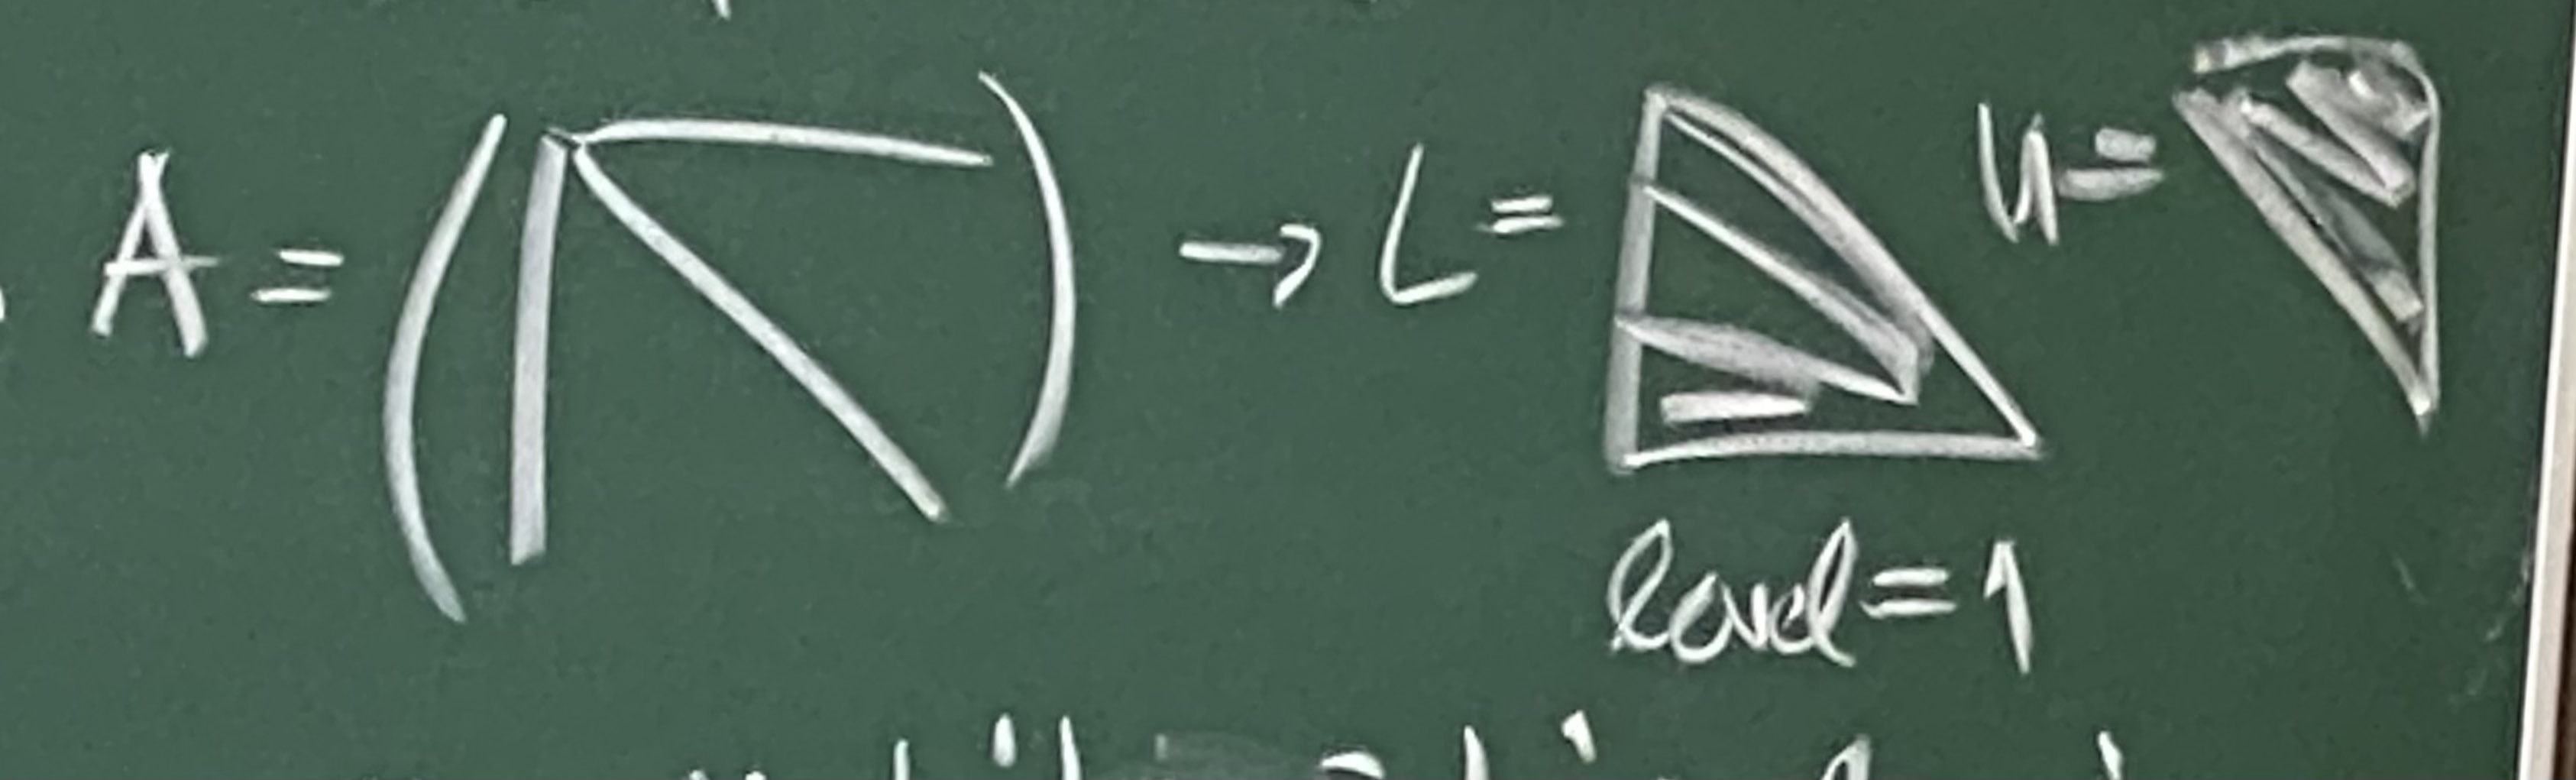
\includegraphics{images/30-11-ILU1.jpg}
    \end{figure}

\end{remark}

\subsection{Další varianty}

Maska P vzniká za běhu v závislosi na velikosti zanedbaných prvků.

Z toho máme neúplnost podle hodnoty, malé hodnoty zanedbáme, velké ponecháme.

Říkáme že $a_{ij}^{(k)}$ je malý pokud \begin{equation*}
    |a_{ij}^(k)| < \alpha ||a_{i,\cdot}^{(k)}, \alpha = 0,01
\end{equation*}

Výhoda je, že se nemůže stát abychom zanedbali velký prvek. 

Nevýhoda je, že struktura L,U závisí na numerických hodnotách $a_{ij}^{(k)}$, může vzniknout úplně nová struktura, mnoho zaplnění.
Proto je potřeba doplnit omezení počtu nenulových prvků na řádek.

Z toho dostáváme ILUT($\alpha, n$) - ILUT with threshold. Obvykle se volí $\alpha = 0.01, n=10$

V algoritmu se pak vybírá n největších prvků  v $|\cdot|$, které splní prahové kritérium.


\begin{remark}
    Existují i varianty ILU, které se snaží kompenzovat zanedbané prvky. MILU, respektive MIC (modified ILU resp. IC).
    V nich se zanedbaný prvek přičte k diagonále.
\end{remark}

\begin{remark}
    Při použití IC(0) + CG je potřeba daleko méně iterací než při použití diagonálního předpodmínění.

    Přesto $\varkappa(\mathbb{M}^{-1} \mathbb{A}) = O(h^{-2})$, počet iterací $O(h^{-1})$.

    Pro MIC + CG $\varkappa(\mathbb{M}^{-1} \mathbb{A}) = O(h^{-1})$. Pak je počet iterací k dosažení zadané přesnosti  $O(h^{-\frac{1}{2}})$.
\end{remark}

\begin{remark}
    V každé iteraci je třeba řešit soustavy $\mathbb{P} \mathbb{A} \mathbb{P}^T$ s maticí $M = LU$, děláme 2 zpětné chody.

    To je silně sekvenční operace, špatně se paralelizuje, lze přeuspořádat rovnice:



\end{remark}




\end{document}